\documentclass[10pt,a4paper]{article}

\usepackage[utf8]{inputenc}
\usepackage[francais]{babel}
\usepackage[T1]{fontenc}
\usepackage{amsmath}
\usepackage{amsfonts}
\usepackage{amssymb}
\usepackage{graphicx}
\usepackage{lmodern}
\usepackage{hyperref}
\usepackage[left=2.7cm,right=2.7cm,top=2cm,bottom=3cm]{geometry}
\usepackage{verbatim}
\usepackage{xcolor}
\usepackage{url}

\hypersetup{
    colorlinks,
    linkcolor={red!50!black},
    citecolor={blue!50!black},
    urlcolor={blue!80!black}
}

\title{
\includegraphics[scale=1]{Art/otb-logo.png}\\
  Guide d'installation OTB\\
  {\small\url{https://www.orfeo-toolbox.org}}
}

\begin{document}

\maketitle

\tableofcontents

\clearpage
\section{Paquet de données}

Le paquet de données pour les TPs peut être téléchargé ici: \url{www.orfeo-toolbox.org/packages/WorkshopData/WorkshopData.zip}.

\section{Windows}

\subsection{QGIS}
Installer QGIS: \url{http://www.qgis.org/fr/site/forusers/download.html}.

\subsection{Ligne de commande}
Installer un environnement minimal de ligne de commande pour Windows. Par exemple
Git for Windows est très facile à installer:
\url{http://git-scm.com/download/win}.

\subsection{OTB et Monteverdi}
Pour installer OTB et Monteverdi, téléchargez le paquet OTB correspondants à
votre architecture (32 ou 64 bits). Si votre machine est 32
bits il s'agit de:

\begin{verbatim}
OTB-6.2.0-Win32.zip
\end{verbatim}

Sinon si votre machine est 64 bits:

\begin{verbatim}
OTB-6.2.0-Win64.zip
\end{verbatim}

Ces archives sont disponibles sur la page
\url{https://www.orfeo-toolbox.org/download/}.
Extraire l'archive zip dans votre répertoire personnel, par exemple dans:\\
\begin{centering}
\texttt{C:{\textbackslash}Utilisateurs{\textbackslash}Martin{\textbackslash}install{\textbackslash}}.
\end{centering}

\subsection{Tester l'installation}
Une fois l'installation terminée, les applications OTB sont accessibles de
plusieurs façons. Vérifier que l'installation est fonctionnelle avec les étapes
suivantes:
\begin{enumerate}

\item Lancer monteverdi avec \texttt{monteverdi.bat} depuis le répertoire
d'installation.

\item Essayer d'ouvrir une image tif avec Monteverdi (voir
figure~\ref{fig:monteverdi}). Une image tif de démo est
disponible ici: \url{https://git.orfeo-toolbox.org/otb-data.git/blob/HEAD:/Examples/QB\_Toulouse\_Ortho\_PAN.tif}.

\item Le navigateur d'application est ensuite accessible depuis "Affichage"
$\rightarrow$ "Navigateur d'OTB-Applications".
(Voir figure \ref{fig:windows-mapla}).

\item Naviguer dans le dossier \texttt{bin} du répertoire d'installation OTB et double cliquer sur le
fichier \texttt{.bat} de l'application à lancer, par exemple:\\
\texttt{Martin{\textbackslash}install{\textbackslash}OTB-6.2.0-win32{\textbackslash}bin{\textbackslash}otbgui\_Rescale.bat}
(Voir figure \ref{fig:windows-otbgui}).

\end{enumerate}

\begin{figure}[h]
  \center
  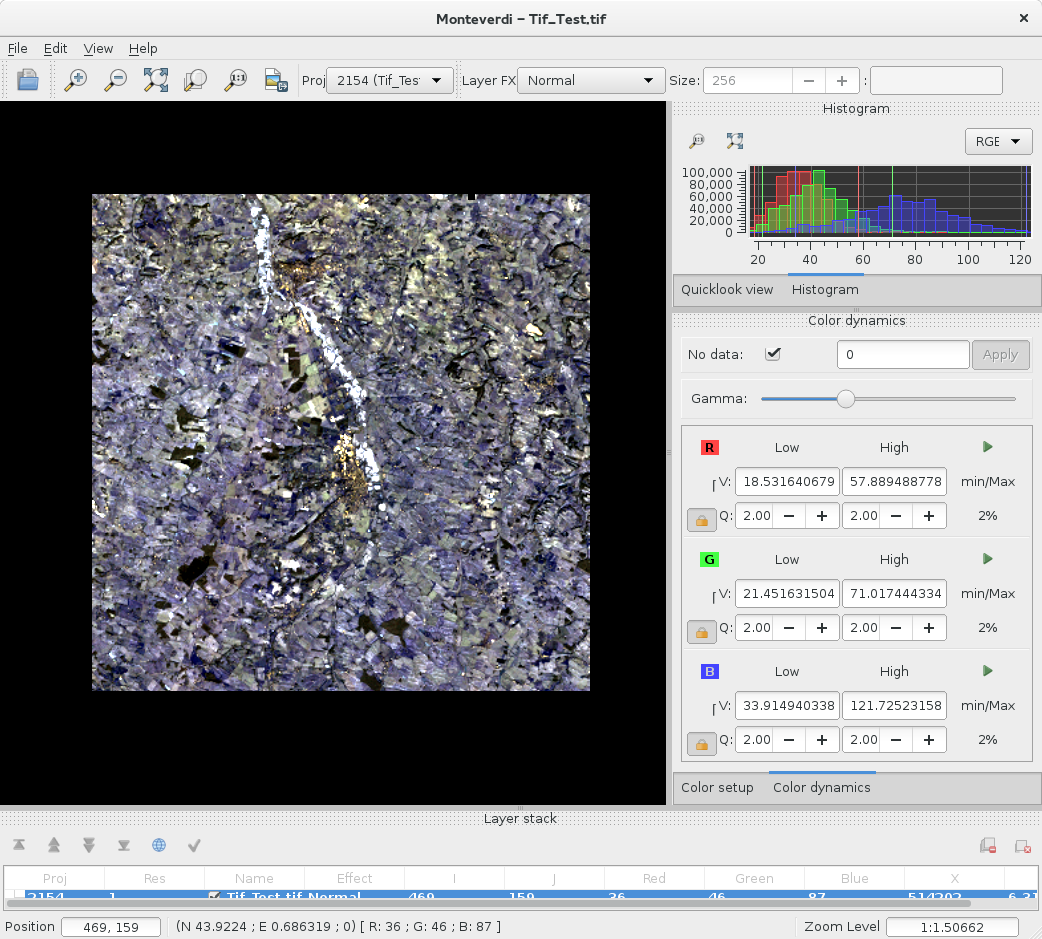
\includegraphics[width=1\textwidth]{Art/monteverdi-tif.png}
  \caption[]{Monteverdi}
  \label{fig:monteverdi}
\end{figure}

\begin{figure}[h]
  \center
  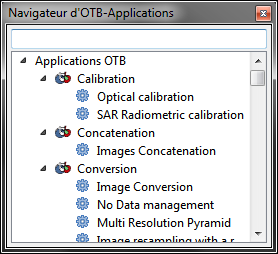
\includegraphics[scale=1]{Art/windows-mapla.png}
  \caption[]{Les applications OTB sont accessibles depuis Monteverdi}
  \label{fig:windows-mapla}
\end{figure}

\begin{figure}[h]
  \center
  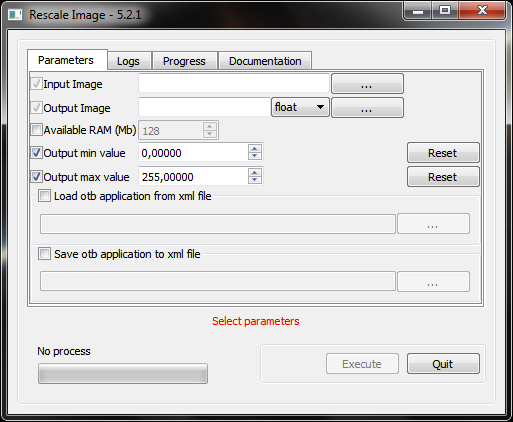
\includegraphics[scale=1]{Art/windows-otbgui.png}
  \caption[]{Interface graphique OTB}
  \label{fig:windows-otbgui}
\end{figure}

% En commentaire pour l'instant, c'est peut être un peu inutile puisqu'il n'y a
% aucune action associée en terme d'installation
\begin{comment}
\subsection{OTB depuis QGIS}

Les applications OTB sont disponibles depuis QGIS. Pour cela

Attention ! QGIS est livré avec ses propres binaires OTB. Les applications ainsi
ouvertes depuis QGIS sont souvent différentes de celles installée ci-dessus, car
il s'agit typiquement d'une version plus ancienne.
Éventuellement, il est possible de remplacer l'OTB livrée avec QGIS en supprimant
ou écrasant les fichiers dans \texttt{}.

\begin{figure}[h]
  \center
  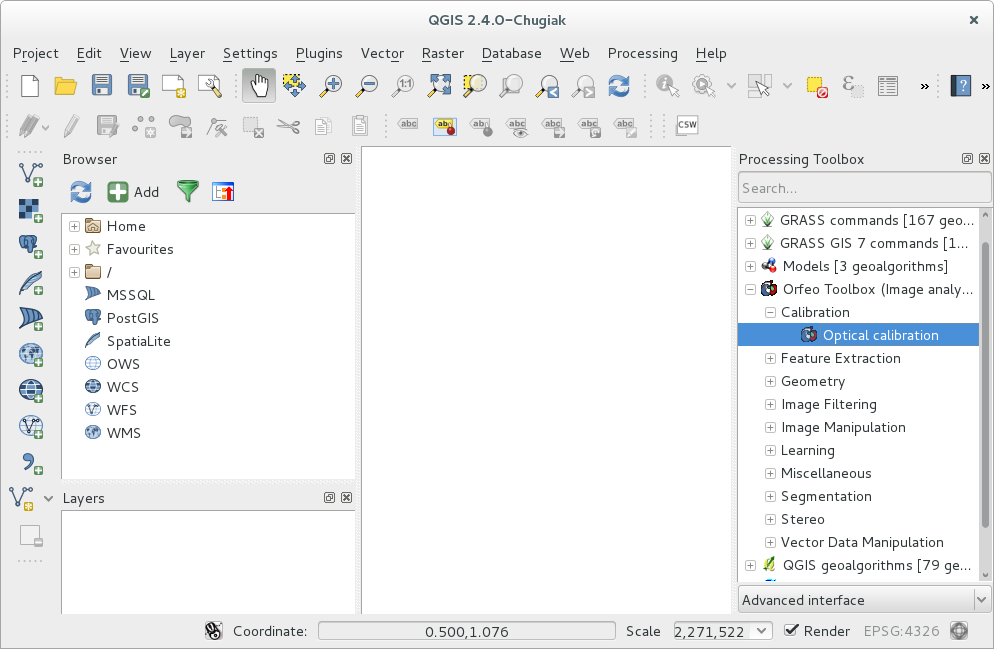
\includegraphics[width=1\textwidth]{Art/qgis-otb.png}
  \caption[]{Intégration QGIS - OTB}
  \label{fig:otb-qgis}
\end{figure}
\end{comment}

\clearpage
\section{Linux (exemple Ubuntu)}

La section ci-dessous détaille la procédure d'installation des outils dans un
environnement Linux (Ubuntu). Cette procédure peut également s'appliquer à
d'autres distributions Linux en adaptant le gestionnaire de paquets (dnf, yum,
emerge, pacman\ldots)

\subsection{QGIS}
QGIS peut être installé via un gestionnaire de paquets graphique ou bien en
ligne de commande, le paquet à installer s'appelle simplement \textbf{qgis}.
\begin{verbatim}
sudo apt-get install qgis
\end{verbatim}

\subsection{Installer les dépendances}
Avant d'installer le paquet autoportant OTB, certaines dépendances système
sont nécessaires. Dans un terminal, taper:
\begin{verbatim}
sudo apt-get install libx11-6 libxext6 libxau6 libxxf86vm1 libxdmcp6 libdrm2
\end{verbatim}
ou équivalent pour d'autres distributions.

Vous aurez en outre besoin des librairies libgl1 et libglu1, qui ont
différentes implémentations (MESA, FGLRX, NVIDIA, ...). Si vous n'avez pas
déjà ces librairies sur votre système, vous pouvez prendre une implémentation
libre comme MESA :
\begin{verbatim}
sudo apt-get install libgl1-mesa-glx libglu1-mesa
\end{verbatim}

\subsection{Installer OTB et Monteverdi}
Télécharger le paquet autoportant OTB pour linux (64 bits), disponible sur la
page:
\begin{center}
\url{https://www.orfeo-toolbox.org/download}
\end{center}

Il s'agit d'une archive auto-extractible, qui va se déployer dans le répertoire
courant. Une fois rendue exécutable, l'archive peut être extraite. Les
exécutables sont dans le sous-dossier 'bin', vous pouvez les rendre facilement
accessible en ajoutant ce chemin au PATH. Les commandes permettant de faire
ce déploiement sont :
\begin{verbatim}
chmod +x OTB-6.2.0-Linux64.run
./OTB-6.2.0-Linux64.run
\end{verbatim}

Il existe ensuite un script permettant de lancer monteverdi ou mapla avec toutes les
variables d'environnement nécessaires:
\begin{verbatim}
cd OTB-6.2.0-Linux64
./monteverdi.sh
./mapla.sh
\end{verbatim}

\subsection{Tester l'installation}
Une fois l'installation terminée, les applications OTB sont accessibles de
plusieurs façons. Vérifier que l'installation est fonctionnelle avec les étapes
suivantes:
\begin{enumerate}

\item Lancer Monteverdi et essayer d'ouvrir une image tif (voir
figure~\ref{fig:monteverdi}). Une image tif de démonstration est disponible ici:
\url{https://git.orfeo-toolbox.org/otb-data.git/blob/HEAD:/Examples/QB\_Toulouse\_Ortho\_PAN.tif}.

\item Le navigateur d'application est ensuite accessible depuis "Affichage"
$\rightarrow$ "Navigateur d'OTB-Applications".
(Voir figure \ref{fig:windows-mapla}).

\item Ouvrir une application OTB via un terminal, par exemple
\texttt{otbgui\_Rescale}. (Voir figure \ref{fig:windows-otbgui}).

\end{enumerate}

\clearpage
\section{Mac OS X}

Les logiciels peuvent également être installés sur un système Mac OS X.

Installer d'abord QGIS en vous référant à la page officiel pour les instructions
relatives au système Mac OS X.

Pour installer OTB et Monteverdi, téléchargez le paquet OTB:

\begin{verbatim}
OTB-6.2.0-Darwin64.run
\end{verbatim}

Cette archive est disponible sur la page \url{https://www.orfeo-toolbox.org/download/}.

Il s'agit d'une archive auto-extractible, qui va se déployer dans le répertoire
courant.

Reportez vous à la section ``Tester l'installation'' de la section ``Linux''
pour vérifier l'installation des logiciels.

\end{document}
